\documentclass[11pt]{article}
\usepackage{amsmath}
\usepackage{graphicx}
%\input{definitions}

\renewcommand{\baselinestretch}{1.2}
\setlength{\topmargin}{-0.25in}
\setlength{\oddsidemargin}{0.50in}
\setlength{\textwidth}{5.9in}
\setlength{\textheight}{8.5in}

\newcommand{\I}{{\bf I}}
%\input{psfig}

\begin{document}

\begin{center}
{\bf Computer Vision I: Low-Middle Level Vision  Homework Exercise \#2 }  \\ (total 15 points)   \\
Due: November 28th 11:59 PM.

2100017727 Keran Wang
\end{center}

\vspace{5mm}

\vspace{5mm}

\noindent{\bf Question 1}. (Minimax entropy learning, 3 points).

\textbf{Answer:}
\begin{enumerate}
    \item
    $$
    Z = \int_{\I}\exp{\left\{-\sum_{i}^{K}<\lambda_i, H_i(\I)>\right\}}\textbf{d}\I
    $$
    Thus,
    $$
    \frac{\partial \log{Z}}{\partial\lambda_i}=\frac{1}{Z}\frac{\partial Z}{\partial \lambda_i}=-E_p[H_i(\I)]
    $$

    \item
    By definition, $\ell(\Theta)=-\log p(\I, \Theta)$, which means
    $$
    \ell(\Theta)=-\log p(\I, \Theta)=-\log Z-\sum_{i=1}^{K}<\lambda_i, H_i(\I)>
    $$
    Due to the nature of inner product, the second term vanishes in the second derivative.
    $$
    \begin{aligned}
    \frac{\partial^2\ell(\Theta)}{\partial\lambda_i\partial\lambda_j} &= -\frac{\partial^2 \log Z}{\partial\lambda_i\partial\lambda_j} \\
                                                                      &= \frac{1}{Z^2}\frac{\partial Z}{\partial \lambda_i}\frac{\partial Z}{\partial \lambda_j} - \frac{1}{Z}\frac{\partial^2 Z}{\partial\lambda_i\partial\lambda_j} \\
                                                                      &= E_p[H_i(\I)]E_p[H_j(\I)]-E_p[H_i(\I)H_j(\I)] \\
                                                                      &= -E_p[(H_i(\I)-h_i)(H_j(\I)-h_j)]
    \end{aligned}
    $$

    \item
    The left hand side of this equation is
    $$
    \begin{aligned}
    LHS &= E_f[\log f] - E_f[\log p] - E_f[\log f] + E_f[\log p_+] \\
        &= E_f[\log p_+] - E_f[\log p] \\
        &= E_f[-\log Z -\sum_{\alpha=1}^{K}<\lambda^*_\alpha, H_\alpha(\I)> - <\lambda_+, H_+(\I)>] - E_f[-\log Z -\sum_{\alpha=1}^{K}<\lambda_\alpha, H_\alpha(\I)>] \\
        &= -\log Z - \sum_{\alpha=1}^{K}<\lambda^*_\alpha, E_f[H_\alpha(\I)]> - <\lambda_+, E_f[H_+(\I)]> + \log Z - \sum_{\alpha=1}^{K}<\lambda_\alpha, E_f[H_\alpha(\I)]> \\
        &= - \sum_{\alpha=1}^{K}<\lambda^*_\alpha, E_{p_+}[H_\alpha(\I)]> - <\lambda_+, E_{p_+}[H_+(\I)]>  - \sum_{\alpha=1}^{K}<\lambda_\alpha, E_{p_+}[H_\alpha(\I)]> \\
        &= E_{p_+}[\log p_+] - E_{p_+}[\log p] = KL(p_+||p)
    \end{aligned}
    $$
\end{enumerate}

\noindent{\bf Question 2}. (Learning by information projection, 3 points).

\textbf{Answer:}
\begin{enumerate}
    \item 
    Here, we are searching for the solution for the constrained problem:
    $$
    p = \arg\min_{p\in\Omega_i}\int p(\I)\log \frac{p(\I)}{q(\I)}\mathrm{d}\I
    $$
    with constraint
    $$
    \int p(\I)H_i(I)\mathrm{d}\I = h_i
    $$
    and
    $$
    \int p(\I)\mathrm{d}\I = 1
    $$
    Using the Lagrarian method, we are optimizing the function:
    $$
    \mathcal{L} = p(\I)\log \frac{p(\I)}{q(\I)} + \sum_{i=1}^{K}\lambda_i p(\I)H_i(I) + \lambda_0 p(\I)
    $$
    We have elimiated the constants useless for optimization.
    Thus, we have
    $$
    \frac{\partial \mathcal{L}}{\partial p} = \log \frac{p(\I)}{q(\I)} + 1 + \sum_{i=1}^{K}\lambda_i H_i(I) + \lambda_0 = 0
    $$
    Correspondingly,
    $$
    p(\I) = \exp{(-1-\lambda_0-\sum_{i = 1}^{K}\lambda_i H_i(\I))}q(\I)
    $$
    \item 
    The left hand side of this equation is
    $$
    \begin{aligned}
    LHS &= E_f[\log f] - E_f[\log q] - E_f[\log f] + E_f[\log p] \\
        &= E_f[\log p] - E_f[\log q] \\
    \end{aligned}
    $$
    Due to the equation of the expect for f and q, we have
    $$
    \begin{aligned}
        LHS &= E_p[\log p] - E_p[\log q] \\
            &= KL(p||q) \\
    \end{aligned}
    $$
    \item When $q(\I)$ is a uniform distribution, the expression can be rewritten as
    $$
    \begin{aligned}
    p &= \arg\min_{p\in\Omega_i}\int p(\I)\log \frac{p(\I)}{q(\I)}\mathrm{d}\I \\
      &= \arg\min_{p\in\Omega_i}\int p(\I)\log {p(\I)}\mathrm{d}\I \\
      &= -\arg\max_{p\in\Omega_i}\int p(\I)\log {p(\I)}\mathrm{d}\I \\
    \end{aligned}
    $$
\end{enumerate}

\noindent{\bf Question 3}. (Information projection, 3 points)

\textbf{Answer:}
\begin{enumerate}
    \item 
    Similar to Quesion 1, here, $\beta_K$ is $\lambda_i$, and $q_{K-1}$ is $p$, thus,
    $$
    \frac{\partial \log z_K}{\partial \beta_K} = E_{q_{K-1}}[h_K(x)]
    $$
    \item 
    Similarly, we have
    $$
    \frac{\partial^2\log Z_K}{\partial\beta_i\partial\beta_j} = E_{q_0}[(h_i(x) - h^{obs}_i)(h_j(x) - h^{obs}_j)]
    $$
    \item Leveraging the equation between $E_f[\cdot]$ and $E_{q_{K+1}}[\cdot]$, the proof is similar.
\end{enumerate}

\noindent{\bf Question 4}. (Typical set, 3 points)

\textbf{Answer:}
\begin{enumerate}
    \item Given $N$, the coin has $qN$ times head up, the number is
    $$
    \#\Omega(q) = {N \choose qN} = \frac{N!}{qN!(N-qN)!}
    $$
    We regard N as a really big number, we have stirling's approximation
    $$
    \#\Omega(q) = \frac{1}{\sqrt{2\pi N q(1-q)}q^{qN}(1-q)^{(1-q)N}}
    $$ 
    Substitute $q$ with 0.2 and 0.5
    $$
    \#\Omega(0.2) = \frac{1}{\sqrt{0.32\pi N}0.2^{0.2N}0.8^{0.8N}}
    $$
    $$
    \#\Omega(0.5) = \frac{1}{\sqrt{\frac{\pi N}{2}}}2^N
    $$
    \item 
    $$
    p(S_N) = p^{qN}(1-p)^{(1-q)N}
    $$
    $$
    p(\Omega(q)) = p(S_N)\#\Omega(q) = \frac{p^{qN}(1-p)^{(1-q)N}}{\sqrt{2\pi N q(1-q)}q^{qN}(1-q)^{(1-q)N}}
    $$
    \item
    When $p\neq q$, one of the two fractions $\frac{q}{p}$ and $\frac{p}{q}$ is lower than 1,
    and with the effect of infinite exponent, the probablity of being obeserved will converge to zero swiftly.
    So, we can observe it if and only if $p = q$.
\end{enumerate}

\noindent{\bf Question 5}. (Poisson Distribution and Random Sampling, 3 points)

\textbf{Answer:}
\begin{enumerate}
    \item 
    \begin{figure}
        \centering
        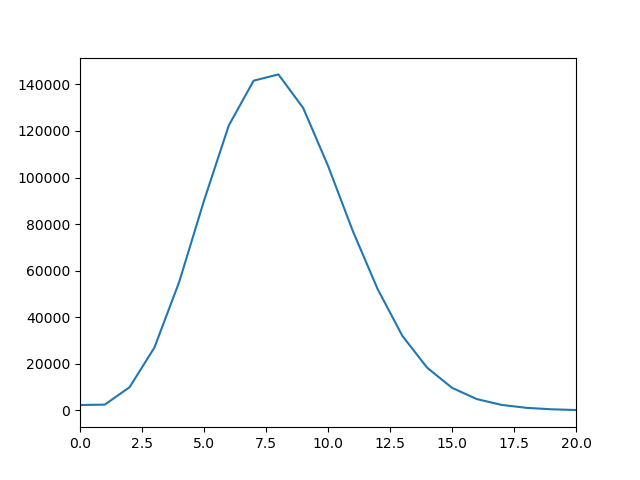
\includegraphics[width=0.5\textwidth]{Figure_1.png}
        \caption{$\lambda = 0.1$, $L = 10$}
    \end{figure}
    \begin{figure}
        \centering
        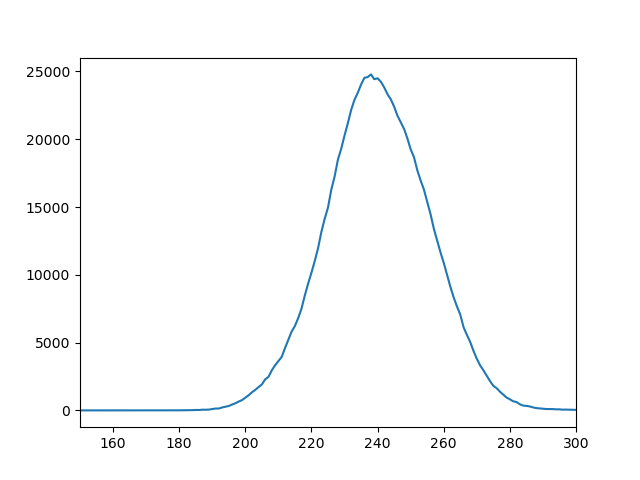
\includegraphics[width=0.5\textwidth]{Figure_2.png}
        \caption{$\lambda = 0.1$, $L = 50$}
    \end{figure}
    \begin{figure}
        \centering
        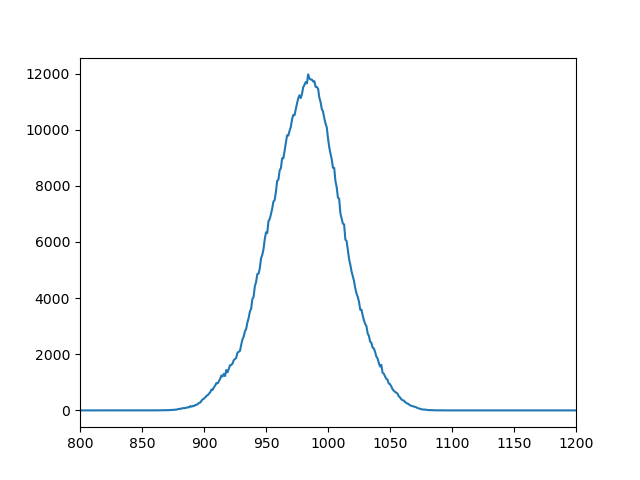
\includegraphics[width=0.5\textwidth]{Figure_3.png}
        \caption{$\lambda = 0.1$, $L = 100$}
    \end{figure}
    \begin{figure}
        \centering
        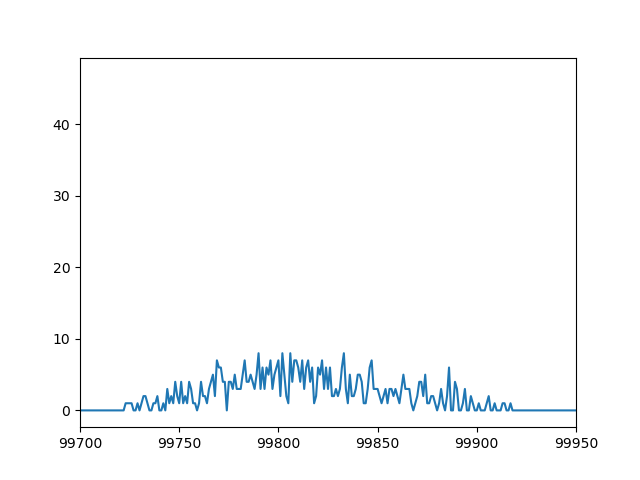
\includegraphics[width=0.5\textwidth]{Figure_4.png}
        \caption{$\lambda = 0.1$, $L = 1000$}
    \end{figure}
    \begin{figure}
        \centering
        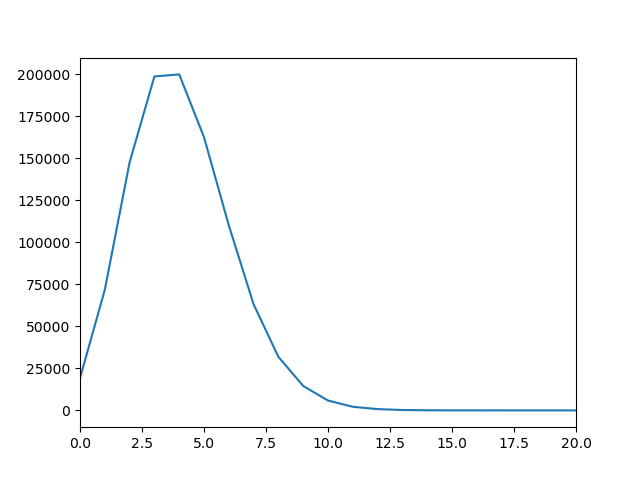
\includegraphics[width=0.5\textwidth]{Figure_5.png}
        \caption{$\lambda = 0.05$, $L = 10$}
    \end{figure}
    \begin{figure}
        \centering
        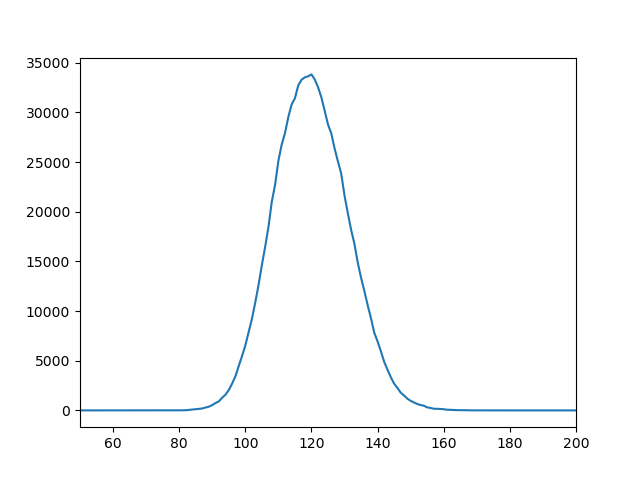
\includegraphics[width=0.5\textwidth]{Figure_6.png}
        \caption{$\lambda = 0.05$, $L = 50$}
    \end{figure}
    \begin{figure}
        \centering
        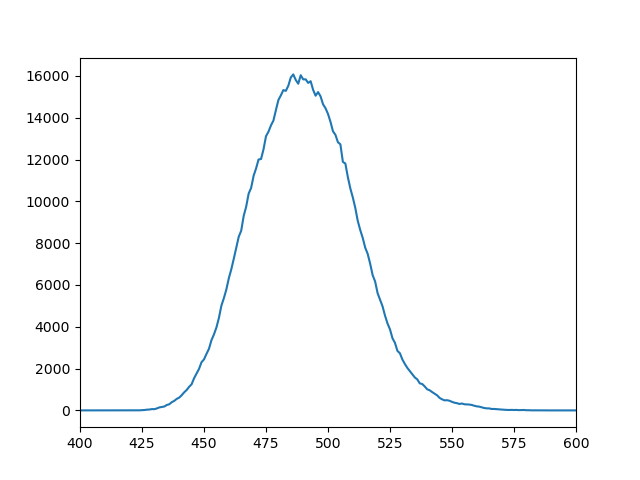
\includegraphics[width=0.5\textwidth]{Figure_7.png}
        \caption{$\lambda = 0.05$, $L = 100$}
    \end{figure}
    \begin{figure}
        \centering
        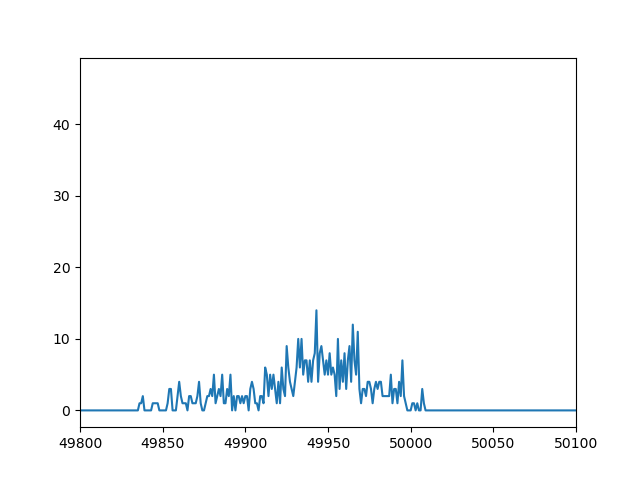
\includegraphics[width=0.5\textwidth]{Figure_8.png}
        \caption{$\lambda = 0.05$, $L = 1000$}
    \end{figure}
    \item 
    The probability for one point in a $l\times l$ square is $\frac{l^2}{n^2}$, and the total probability is binom distribution:
    $$
    P_s(k) = {N \choose k}(\frac{l^2}{n^2})^k(1-\frac{l^2}{n^2})^{N-k}
    $$
    When $\frac{l^2}{n^2}$ is very small, we can have an approximation:
    $$
    (1-\frac{l^2}{n^2})^{N-k}=\exp{(-\frac{(N-k)l^2}{n^2})}
    $$
    So, we got
    $$
    P_s(k) = \frac{(N\frac{l^2}{n^2})^k}{k!}e^{-\frac{Nl^2}{n^2}}
    $$
    Notice that $N=\lambda l^2$, this is exact the Poisson Distribution
\end{enumerate}
\end{document}